\chapter{Il teorema di Cauchy-Kowalevski} \label{invariant}

Adesso che abbiamo sviluppato tutti gli strumenti necessari, ipotizziamo di avere un problema di Cauchy qualsiasi. Come abbiamo mostrato nel paragrafo \ref{pb}, esso può essere riscritto nella forma:
$$
\begin{cases}
F(x,t, D^\alpha_x D^j_t u)=0 & |\alpha | +j \leq k\\
D^j_t u (x,0)= \phi_j(x) & \text{per }j<k 
\end{cases}
$$
Di conseguenza ci occuperemo solo di quest'ultimo caso, in cui le condizioni vengono assegnate su $\Gamma_0=\{ t=0 \}$.

L'assunzione fondamentale di questo capitolo è che i dati ($F$ e $\phi_j$) siano analitici in un intorno dell'origine, proprietà che utilizzeremo per mostrare l'esistenza di un'unica \textbf{soluzione analitica}, sempre in intorno dell'origine.

Per garantire l'esistenza, però, siamo costretti a fare qualche ipotesi sulla struttura dell'equazione. 
Considerando quanto è stato detto nel capitolo precedente, soprattutto per quanto riguarda il teorema \ref{teoescar}, l'intuito suggerisce che potrebbe essere una buona idea considerare che la superficie $\Gamma_0$ sia \textbf{non caratteristica}. 
Tale proprietà ci permette di riscrivere nuovamente l'equazione in un'altra forma, ancora più semplice, ovvero:
\begin{equation}\label{pbnorm}
\begin{cases}
D_{t}^k u = G(x,t, D^\alpha_x D^j_t u) & |\alpha |+ j \leq k, \, j<k \\
D_t^ju = \phi_j & \text{ su } \Gamma_0, \, j<k
\end{cases} \\
\end{equation}
Questa idea ci permetterà di dimostrare il TCK.
\begin{namedtheorem}[Teorema di Cauchy-Kowalevski]
\hpth{
\text{Problema \eqref{pbnorm}}\\
G, \, \phi_j \text{ analitici in intorno dell'origine}
}
{\exists ! \; u \text{ soluzione analitica in intorno dell'origine}}
\end{namedtheorem}


Dopo aver mantenuto uno sguardo quanto più generale possibile, ci vogliamo occupare di capire come dimostrare il risultato che abbiamo in mente. L'approccio che seguiremo sarà ``al contrario'', ovvero generalizzando progressivamente i risultati. Infatti, partiremo dal caso meno generale, fino ad arrivare a quello di un'equazione in forma normale, seguendo di fatto l'ordine cronologico dei risultati.




\newpage
\section{EDO}

Per prima cosa affrontiamo un teorema molto simile al TCK, che tratta il caso di un sistema di EDO in forma normale.
Cominciamo subito col riportare l'enunciato.

\begin{theorem}\label{teoedo}
\hpth{
A \subseteq \mathbb{C}, \, B\subseteq \mathbb{C}^n \text{ aperti }\\
\Omega \subseteq A \text{ aperto connesso}\\
f:A\times B\rightarrow\mathbb{C}^n \text{ olomorfa}\\
\text{Pb: }
\begin{cases}
y' = f(x,y) \quad \forall x \in \Omega \\
y(x_0)=y_0
\end{cases}\\
}
{
\text{localmente esiste un'unica soluzione olomorfa}
}
\end{theorem}

\begin{remark}
Non esclude la possibilità di trovare altre soluzioni non analitiche.
\end{remark}

Questo risultato fu la prima applicazione della teoria delle funzioni olomorfe in combinazione con il metodo dei maggioranti, la quale, come già sappiamo, è stata proposta da Cauchy nella prima metà dell'Ottocento.
Non riportiamo la dimostrazione per esteso, perché utilizza un maggiorante diverso rispetto a quello che abbiamo introdotto nel paragrafo \ref{seriedipotenze} (ovvero quello che utilizzeremo per dimostrare il TCK). 
In ogni caso, può essere trovata in \cite{Delf} e la struttura del ragionamento è la stessa del teorema \ref{teoquasilin}.

Nonostante non affrontiamo la questione dell'esistenza nel dettaglio, è conveniente discutere a parole e in modo esaustivo il problema dell'\textbf{unicità} di soluzioni analitiche (o olomorfe). Una funzione analitica è univocamente determinata da tutte le sue derivate in un punto, le quali, in questo caso, sono note grazie all'analiticità della funzione $f$.
Chiudiamo completamente il discorso affrontando anche la situazione di una EDP: anche qui, assumendo i dati analitici, è possibile conoscere tutte le derivate parziali della funzione, grazie al fatto che la superficie su cui vengono assegnate le condizioni è assunta non caratteristica.

Poiché questo risultato è stato dimostrato costruendo un maggiorante per la soluzione $y$, è possibile ottenere una stima del suo raggio di convergenza sfruttando il teorema \ref{teomagg}.

\begin{theorem}
\hpthml{
\text{Ipotesi del teorema \ref{teoedo}}\\
\exists \, \overline{B_a(x_0)}\subseteq A,\,\overline{B_b(y_0)} \subseteq B\\
M=\max_{B_a(x_0),\, B_b(y_0)}|f|
}{
\text{La soluzione ha raggio almeno } \widetilde{r}= a\left[ 1-\exp\left( -\frac{b}{aM(n+1)}\right) \right] 
}
\end{theorem}

\begin{remark}
E' interessante notare cosa accade quando $B=\mathbb{C}^n$.
\end{remark}




\newpage
\section{EDP quasi-lineari}

Ora è il momento di trattare la chiave di volta di tutto il ragionamento sulle EDP, ovvero il teorema che mostra l'esistenza, e quindi anche l'unicità, di una soluzione analitica di un sistema quasi-lineare di EDP in forma normale.

\begin{theorem}\label{teoquasilin}
\hpth{
A_i , \, B\text{ analitici in un intorno dell'origine }\\
\text{Pb: }
\begin{cases}
D_t \, y = \sum\limits_{i=1}^{n-1} A_i(x,y)D_{x_i}y+B(x,y) \; \\
y=0 \quad \text{ su } \Gamma_0
\end{cases}
\\
}{
\exists ! \; y(x,t): \mathbb{R}^n \rightarrow \mathbb{R}^m
\text{ sol. analitica in intorno dell'origine}
}
\end{theorem}

\begin{remark}
Questo teorema può essere tranquillamente modificato sostituendo l'analiticità con l'\textbf{olomorfia}, in modo da ottenere un enunciato simile al caso delle EDO, poiché l'estensione è immediata, in quanto nella dimostrazione non si fa alcuna particolare assunzione che distingue il caso reale da quello complesso.
\end{remark}



\begin{proof}
Prima di tutto chiamiamo $a^i_{ml}$ le componenti di $A_i$  e $b_m$ quelle di $B$, mentre i coefficienti delle serie rispettivamente $(a^i_{ml})_\gamma$ e $(b_m)_\gamma$. Ora procediamo per punti.
\begin{enumerate}
\item Ragionando componente per componente, ipotizziamo $y_h = \sum c^h_{\alpha j} x^\alpha t^j$ con ${h=1,\ldots, m}$.
\item La condizione di Cauchy ci dice che $c^h_{\alpha 0}=0$.
\item Inserendo le serie di $y,\, A_i,\, B$ nell'equazione e utilizzando i teoremi \ref{composizione}, \ref{derivata} e \ref{prodotto}, si ottiene per ogni riga $h$ l'equazione:
$$\sum\limits_{\alpha, \, j} (j+1)c^h_{\alpha (j+1)}\, x^\alpha t^j = \sum\limits_{\alpha,\, j} P_{\alpha j}\left((c^h_{\alpha l})_{l\leq j},(a^i_{ml})_\gamma, (b_m)_\gamma\right) \, x^\alpha t^j$$
dove i polinomi $P_{\alpha j}$ sono naturalmente a coefficienti non negativi.
\item Grazie a questa operazione, ricaviamo una formula ricorsiva per i coefficienti:
$$ c^h_{\alpha (j+1)}= (j+1)^{-1} P_{\alpha j}\left((c^h_{\alpha l})_{l\leq j},(a^i_{ml})_\gamma, (b_m)_\gamma\right),$$
che ci permette di concludere che $c^h_{\alpha j} = Q_{\alpha j}\left((a^i_{ml})_\gamma, (b_m)_\gamma\right)$ dove $Q_{\alpha j}$ sono sempre polinomi a coefficienti non negativi, la cui forma non dipende da $A_i$ e $B$. Allora possiamo anche dire che è sempre possibile costruire una serie di potenze che soddisfa l'equazione. Ci resta da capire se essa converge con un raggio positivo.
\newpage
\item Supponiamo ora di avere un altro problema con la stessa struttura definito dalle funzioni $\widetilde{A}_i $ e $\widetilde{B}$ e di conoscere una sua soluzione analitica locale $\widetilde{y}$. Vogliamo mostrare che $$\widetilde{A}_i \gg A_i, \, \widetilde{B} \gg B \implies \widetilde{y} \gg y.$$
Tenendo in considerazione che per entrambi i problemi valgono le stesse considerazioni fino al punto 4 (i polinomi $Q_{\alpha j}$ sono gli stessi!), possiamo scrivere la seguente catena di disuguaglianze:
\begin{align*}
\left|c^h_{\alpha j}\right| &= \left|Q_{\alpha j}\left((a^i_{ml})_\gamma, (b_m)_\gamma\right)\right|\\
&\leq Q_{\alpha j}\left(\left|(a^i_{ml})_\gamma\right|, \left|(b_m)_\gamma\right|\right) 
& \text{coeff. non negativi}\\
&\leq Q_{\alpha j}\left((\widetilde{a}^i_{ml})_\gamma, (\widetilde{b}_m)_\gamma\right) = \widetilde{c}^h_{\alpha j}
& \widetilde{A}_i \gg A_i, \, \widetilde{B} \gg B
\end{align*}
\item L'ultimo passo consiste nello scegliere $\widetilde{A}_i, \, \widetilde{B}$, in modo tale da poter calcolare esplicitamente $\widetilde{y}$ e poter mostrare che essa è analitica. Viste le nostre conoscenze sulle serie di potenze che arrivano dal teorema \ref{costrmagg}, sappiamo costruire un maggiorante per $A_i$ e $B$. Quindi, selezioniamo due costanti $C$ ed $r$ in modo tale che 
$$\frac{Cr}{r-(x_1+\ldots +x_{n-1})-(y_1+\ldots +y_m)}=\mathcal{M}_{Cr}(x,y) \gg A_i(x,y),\, B(x,y)$$
e che soddisfino le disequazioni \eqref{r} e \eqref{C}. Definiamo quindi il problema
\begin{equation*}
\begin{cases}
D_t \, \widetilde{y}_h = \mathcal{M}_{Cr} (x,y) \left[\sum\limits_{i,\, j} D_{x_j}\widetilde{y}_i+1 \right] \\
\widetilde{y_h}=0 \quad \text{ su } \Gamma_0
\end{cases}
\end{equation*}
dove $h=1,\ldots, m$. A questo punto è possibile dimostrare, utilizzando il metodo delle caratteristiche per equazioni quasi-lineari del primo ordine (paragrafo \ref{metodocar}), che esso ha come soluzione
\begin{equation}\label{maggiorante}
\widetilde{y}_h(x,t)=u(x_1+\cdots +x_{n-1},\,t) \quad \forall h
\end{equation}
dove
\begin{equation}\label{sol}
u(s,t)=\frac{r-s-\sqrt{(r-s)^2-2tCrmn}}{mn},
\end{equation}
la quale è chiaramente analitica in intorno dell'origine. Si veda \cite[cap.1]{Folland} per il completo svolgimento del calcolo.
\item Concludiamo osservando un fatto interessante: non c'è niente di specifico che garantisca che la soluzione trovata continui a garantire la maggiorazione. Infatti, è importante verificare che $\widetilde{y}$ soddisfi la disuguaglianza $|(x,\widetilde{y}(x,t))|< r$ (in modo che $\mathcal{M}_{Cr}$ sia effettivamente una serie di potenze). Per maggiori dettagli si veda la proposizione \ref{prop}.
\end{enumerate}
\end{proof}

\newpage

Come nel caso del sistema di EDO, se sfruttiamo il teorema \ref{teomagg}, possiamo stimare il raggio di convergenza, studiando il raggio della soluzione maggiorante in \eqref{maggiorante}. 

\begin{theorem}\label{stimaraggio}
La soluzione del teorema \ref{teoquasilin} converge con raggio almeno
$$\widetilde{r} = \dfrac{1}{n-1}\, \dfrac{r}{8Cmn} \text{ con } C \geq \frac{1}{2}$$
\end{theorem}
\begin{remark}
$n \geq 2$ affinché il sistema sia realmente alle derivate parziali. 
\end{remark}
\begin{remark}
E' interessante soffermarsi sull'andamento rispetto a $r$, sapendo che:
\begin{align}\label{r}
r <& \min \{ \textit{raggi di conv. dei coefficienti } a^i_{ml}, \, b_m\} \\
\label{C}
C \geq & \max \begin{Bmatrix}
\max\limits_{i,m,l,\alpha } \left| (a^i_{ml})_\alpha \, r^{|\alpha |}\right|\\
\max\limits_{m,\alpha} \left|(b_m)_\alpha \, r^{|\alpha |}\right|
\end{Bmatrix}
\end{align}
\end{remark}


\begin{proof}
Fissiamo $r$ e $C$ come sopra, inoltre ipotizziamo che $C\geq 1/2$ (possiamo farlo senza alcun problema). 
Inizialmente ci concentriamo sulla funzione in \eqref{sol}, la quale è analitica in un intorno dell'origine, in particolare nell'insieme 
$$A = \left\{ (s,t) \in \mathbb{R}^2 : t<\frac{(r-s)^2}{2Crmn} \right\} .$$
Ovvero è sviluppabile in serie di potenze in $B_l(0)$ con $0<l<d=\text{dist}(0, \partial A)$.
\begin{center}
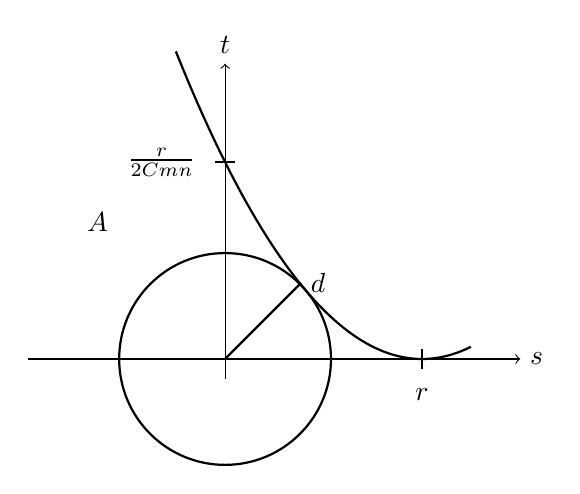
\begin{tikzpicture}[scale=2.5]
    % Disegna il cerchio con centro in (0,0) e raggio 0.538
    \draw[thick,black] (0,0) circle[radius=0.538];
    
    % Disegna la parabola y = (1-x)^2
    \draw[thick,black,domain=-0.25:1.25,samples=100] 
        plot ({\x}, {(1-\x)^2});
    
    \node[black,anchor=south west] at (-0.75, 0.60) {$A$};
    
    % Disegna gli assi
    \draw[->] (-1,0) -- (1.5,0) node[right] {$s$};
    \draw[->] (0,-0.1) -- (0,1.5) node[above] {$t$};
    
    % Disegna il segmento da (0,0) a (sqrt{0.538/2}, sqrt{0.538/2})
    \draw[thick,black] (0,0) -- (sqrt{0.538/1.9},sqrt{0.538/1.9});
    \node at (sqrt{0.538/1.9},sqrt{0.538/1.9}) [right] {$d$};
    
    % Disegna le tacchette richieste
    \draw[thick] (1, 0.05) -- (1, -0.05); % Tacchetta in (1, 0)
    \node at (1, -0.1) [below] {$r$};    % Etichetta per (1, 0)
    
    \draw[thick] (-0.05, 1) -- (0.05, 1); % Tacchetta in (0, 1)
    \node at (-0.1, 1) [left] {$\frac{r}{2Cmn}$}; % Etichetta per (0, 1)
    
\end{tikzpicture}
\end{center}
Scegliendo $l_1 = (n-1)\,\widetilde{r}$ si può dimostrare che, per $C>1/8$, si ha effettivamente che $l_1<d$. L'obiettivo sarebbe, quindi, verificare che $$\sqrt{l_1^2-s^2} < \frac{(r-s)^2}{2Crmn}$$ per ogni $|s|<l_1$, ma ciò è implicato da 
\begin{equation} \label{l1}
l_1 < \frac{(r-l_1)^2}{2Crmn}\; ,
\end{equation}
disuguaglianza che risulta vera se e solo se $C > 1/(4mn) \leq 1/8$.

Ora, invece, ci occupiamo di generalizzare questa cosa per la funzione $\widetilde{y}_h$ in \ref{maggiorante} con $h$ fissato. Essa è analitica nella regione 
$$A = \left\{ (x,t) \in \mathbb{R}^n : t<\frac{(r-(x_1+\ldots +x_{n-1}))^2}{2Crmn} \right\} .$$
La struttura del problema risulta la stessa, quindi, naturalmente, la definizione di $d$ resta invariata. L'unico aspetto che dobbiamo curare è che, in questa situazione, sarà necessario scegliere $l_2 =\widetilde{r}$. 
Quindi, vogliamo mostrare che $$\mathcal{L}=\sqrt{l_2^2-(x_1^2+\ldots +x_{n-1}^2)} < \frac{(r-(x_1+\ldots +x_{n-1}))^2}{2Crmn}=\mathcal{R}$$
quando $|x|=|(x_1,\ldots ,x_{n-1})|< l_2$. Ma ciò è implicato dalla disequazione \ref{l1}, che sappiamo essere vera. Dimostriamolo in due passi.
\begin{itemize}
\item Vale che $\mathcal{L}^2< l_2^2 \leq l_1^2$ per $|x|< l_2$.
\item Vale che $$\left(\frac{(r-l_1)^2}{2Crmn}\right)^2 \leq \min \left\{ \mathcal{R}^2 : |x|\leq l_2 \right\}< \mathcal{R}^2 \, \text{ per } \, |x|< l_2.$$
Lo si mostra sapendo che $$\max \left\{ x_1+\ldots +x_{n-1} : |x|\leq l_2\right\}= (n-1)\frac{l_2}{\sqrt{n-1}}\leq l_1$$ e facendo vedere che $r-(x_1+\ldots +x_{n-1})>0$ per $|x|\leq l_2$ con la disuguaglianza triangolare.
\qedhere
\end{itemize}
\end{proof}

\noindent\rule[0.5ex]{\linewidth}{0.2pt}

Un lettore attento sicuramente si chiederà la ragione dietro alla scelta di un costante $C\geq 1/2$. Ebbene, questo problema emerge da ciò che è stato lasciato aperto nella dimostrazione del teorema \ref{teoquasilin}, ovvero il fatto che in realtà la soluzione $\widetilde{y}$ è veramente maggiorante solo se $|(x,\widetilde{y}(x,t))|< r$. Tale proprietà è proprio garantita in una palla di raggio $\widetilde{r}$. Vediamolo con una proposizione che, oltre a chiarire, completa il quadro logico delle dimostrazioni.
\begin{namedtheorem}[Proposizione]\label{prop}
La maggiorazione di $\widetilde{y}$ vale in $B_{\widetilde{r}}(0)$, ovvero
$$|(x,t)|<\widetilde{r} \implies |(x,\widetilde{y}(x,t))|=x_1^2 + \ldots + x_{n-1}^2 + m \, u^2(x_1 + \ldots + x_{n-1},t) < r^2$$
\end{namedtheorem}
\begin{proof}
Per semplicità dimostriamo che $$|(s,t)|< l=(n-1)\,\widetilde{r} \implies s^2 + m \, u^2(s,t) < r^2.$$ La generalizzazione è banale se ci si ispira alla dimostrazione del teorema \ref{stimaraggio}. 
\newpage
Tenendo in considerazione che $|t|,|s|<l<r$ e che $s^2+t^2<l^2=r/(8Cmn)$, scriviamo la seguente catena di disuguaglianze.
\begin{align*}
& s^2 + m \left[ \frac{r-s-\sqrt{(r-s)^2-2tCrmn}}{mn} \right]^2\\ 
&\leq s^2 + \frac{1}{mn^2} \left[ (r-s)^2 + |(r-s)^2-2tCrmn| \right] 
&\begin{system}
\left|s\right| < r \Rightarrow r-s > 0\\
 \sqrt{(r-s)^2 - 2t Cr mn} > 0 
\end{system}\\
&\leq s^2 + \frac{2}{mn^2} (r-s)^2 + \frac{2|t|Crmn}{mn^2} \\
&\leq l^2 + \frac{2}{mn^2} \left( r^2 + l^2 + 2rl \right) + \frac{2lCrmn}{mn^2} 
&\begin{system}
\left|s\right| < l \Rightarrow (r-s)^2 < (r+l)^2\\
\left|t\right| < l
\end{system}\\
&= \left( \frac{r}{8Cmn} \right)^2 + \frac{2r^2}{mn^2} \left[ 1+\frac{1}{(8Cmn)^2} + \frac{1}{4Cmn} + \frac{1}{8} \right] \\
&< r^2 \underbrace{\frac{2}{mn^2} \left[ \frac{r}{8} + \frac{1}{(8C)^2 mn^2} + \frac{r}{(8Cmn)} + \frac{r}{4Cmn} + \frac{1}{8} \right]}_{<1} < r^2 \\
\end{align*}
In particolare l'ultima affermazione vale poiché
\begin{align*}
n \geq 2 \Rightarrow \frac{2}{mn^2} \left(\ldots\right) 
&\leq \frac{1}{2} \left(\frac{9}{8} + \frac{2}{(8C)^2} + \frac{1}{8C}\right) \\
& \leq \frac{1}{2} \left(\frac{9}{8} + \frac{3}{8C}\right) & C>1/8\\
& \leq \frac{3}{16} \left(3 + \frac{1}{C}\right) < 1 & \Leftarrow C \geq \frac{1}{2} 
\end{align*}
\end{proof}

\newpage
\section{EDP in forma normale}
Ora ci occupiamo di sfruttare i risultati del paragrafo precedente per generalizzare quel risultato al caso di un'equazione in forma normale. Per fare ciò, è sufficiente enunciare e dimostrare il seguente teorema.
\begin{theorem}\label{teonorm}
I due problemi seguenti sono equivalenti
\begin{align*}
\text{non-lineare : }&
\begin{cases}
D_{t}^k u = G(x,t, D^\alpha_x D^j_t u) & |\alpha |+ j \leq k, \, j<k \\
D_t^ju = \phi_j & \text{ su } \Gamma_0, \, j<k
\end{cases} \\
\text{quasi-lineare : }&
\begin{cases}
D_t \, y = \sum\limits_{i=1}^{n-1} A_i(x,y)D_{x_i}y+B(x,y) \; \\
y=0 \quad \text{ su } \Gamma_0
\end{cases}
\end{align*}
\end{theorem}

\begin{proof}
si divide il ragionamento in tre passi:
\begin{enumerate}
\item si costruisce il sistema in modo tale che $y_{\alpha j}= D^\alpha_x D^j_t u$. \\
Quindi, le matrici $A_i$ e $B$ saranno ricavabili dalle espressioni
\begin{align*}
D_t y_{\alpha j} =& y_{\alpha (j+1)} & |\alpha| + j < k \\
D_t y_{\alpha j} =& D_{x_l} y_{(\alpha-e_l)(j+1)} & |\alpha| + j = k, \; j < k\\
D_t y_{0k} =& D_tG + \sum_{|\alpha|+j < k} D_{y_{\alpha j}}G y_{\alpha (j+1)} \\
& + \sum_{|\alpha|+j = k, \; j < k} D_{y_{\alpha j}} G D_{x_l} y_{(\alpha-e_l)(j+1)}
\end{align*}
dove $l(\alpha)=\min\{ l:\alpha_l\neq 0 \} $, e i dati di Cauchy saranno
\begin{align*}
y_{\alpha j}(x, 0) = & D_x^{\alpha} \phi_j(x) & j < k\\
y_{0k}(x, 0) = & G\left( x, 0, D_x^{\alpha} \phi_j(x) \right) & \lvert \alpha \rvert + j \leq k, \; j < k
\end{align*}
\item si rimuovono le condizioni $\phi$, ridefinendo $y(x,t)\leftarrow y(x,t)-\phi (x)$.
\item si rimuove la dipendenza da $t$, aggiungendo la variabile $y^0=t$, insieme all'equazione $D_t y^0=1$ e al dato $y^0(x,0)=0$.
\end{enumerate}
Concludiamo dicendo che, ovviamente, se $u$ è soluzione del problema in forma normale, le $y_{\alpha j}$ saranno soluzione del problema appena costruito. Ma per dimostrare che la $y_{(0,\ldots,0)}$ (soluzione di quest'ultimo) è anche soluzione del problema in forma normale sono necessari diversi conti che possono essere trovati per esteso in \cite[cap.1]{Folland}.
\end{proof}

\begin{remark}
Ci sono tre aspetti, che emergono anche dalla dimostrazione, su cui è il caso di soffermarsi brevemente a riflettere:
\begin{itemize}
\item mettendo insieme le considerazioni fatte all'inizio del capitolo e i teoremi \ref{teoquasilin} e \ref{teonorm}, segue in modo immediato il TCK;
\item continua a valere la stima del raggio di convergenza;
\item questo teorema di equivalenza si generalizza in modo immediato al caso di un sistema in forma normale.
\end{itemize}
\end{remark}








